\section{Background}
\label{sec_background}








\subsection{DL Workloads and Their Characteristics}
\label{sec_characteristics}


A DL development pipeline typically consists of three stages: data processing, model training and model inference. In this survey, we narrow down our focus to training and inference workloads which account for the most computation and consume the majority of resources in the datacenter.

\begin{figure*}[t]
    \centering
    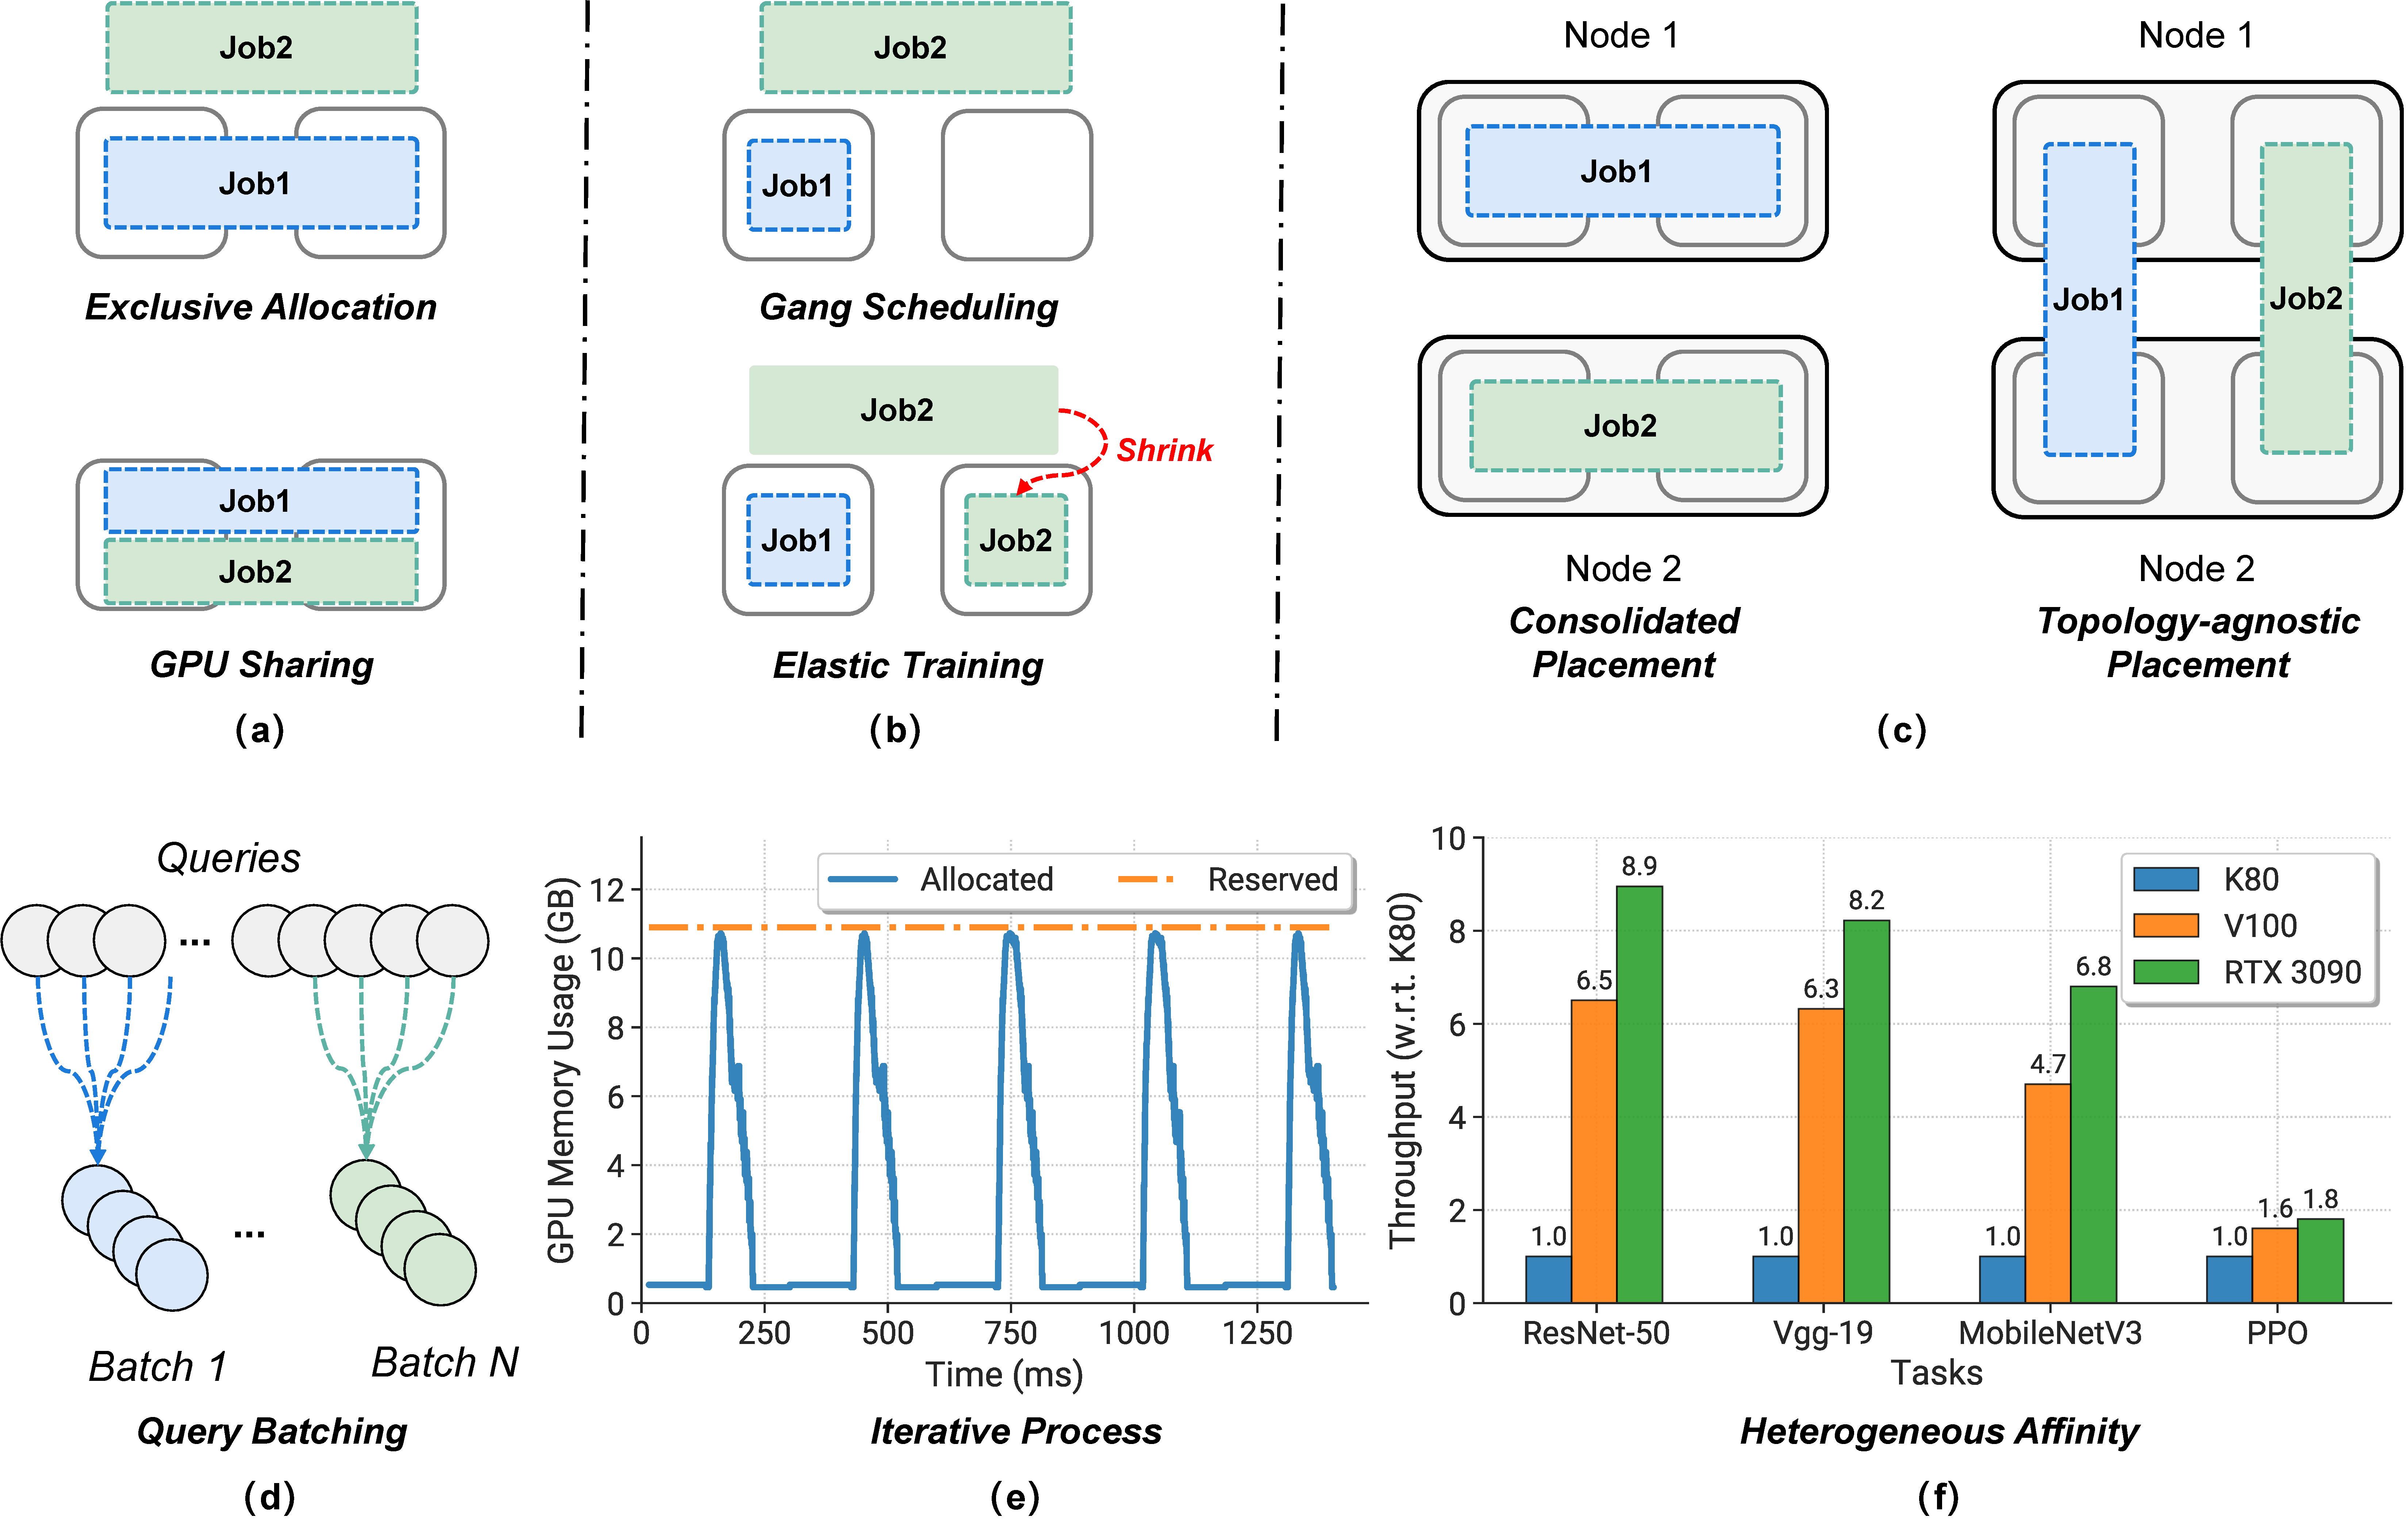
\includegraphics[width=0.95\textwidth]{fig/illustration}
    \vspace{-5pt}
    \caption{\textbf{Characteristics of training and inference workloads.} (\textbf{a}) Exclusive Allocation versus GPU Sharing. (\textbf{b}) Gang Scheduling versus Elastic Training. (\textbf{c}) Consolidated Placement versus Topology-agnostic Placement. (\textbf{d}) Query Batching mechanism in inference. (\textbf{e}) Iterative Process: allocated and reserved GPU memory trace profiled through \texttt{torch.profiler} (ResNet-50 ImageNet classification task). (\textbf{f}) Heterogeneous Affinity: the magnitude of speedup across GPU generations varies significantly across different tasks. }
    \vspace{-15pt}
    \label{figure_illustrate}
\end{figure*}



\subsubsection{DL Training.}
\label{sec:training-feature}
A DL training workload builds models by extracting features from existing data. A DL framework (e.g., PyTorch \cite{PyTorch}, TensorFlow \cite{TensorFlow}) is commonly adopted to fully utilize heterogeneous compute resources to accelerate the training process. To further reduce the training time, the workload is deployed across multiple GPUs with a data-parallel training scheme, which is implemented via distributed training libraries (e.g., Horovod \cite{Horovod}, \texttt{DistributedDataParallel} in Pytorch, \texttt{MultiWorkerMirroredStrategy} in Tensorflow).

DL training workloads exhibit some unique features compared to traditional big data or HPC jobs, which need to be particularly considered for GPU datacenter scheduling. A series of studies have characterized training workloads from the production GPU datacenters, including  Microsoft \cite{Philly}, SenseTime \cite{Helios} and Alibaba \cite{AliPAI, MLaaS}. The characteristics are summarized as below.

\textbf{T1: Inherent heterogeneity} \cite{Philly, Gandiva}. GPU resources play a dominant role in DL training. However, CPUs and memory might interfere with the input processing and then delay the training execution. A GPU datacenter generally offers an ample pool of CPU and memory resources compared to GPUs. Arbitrary selection of heterogeneous resource combinations by users may lead to imperfect training progress. Figure \ref{figure_illustrate} (f) shows the training performance speedups of common DL models with various generations of GPUs. Different models have diverse affinities to GPU types. 


\textbf{T2: Placement sensitivity} \cite{Gandiva,Themis}. Distributed DL jobs are sensitive to the locality of allocated GPU resources. Specifically, the runtime speed of some distributed DL jobs are bounded by device-to-device communication. Figure \ref{figure_illustrate} (c) shows two types of placement, where a consolidated placement can efficiently reduce the communication overhead compared with topology-agnostic placement. The communication sensitivity of training jobs depends on the inherent property of the model structure. Advanced interconnect link (e.g., NVlink) can offer an order of magnitude higher bandwidth than PCIe. Therefore, distributed training jobs tend to request advanced interconnect to further obtain communication time reduction. Besides, jobs colocated in one server may suffer from PCIe bandwidth contention.

\textbf{T3: Iterative process} \cite{Optimus, Chronus}. DL training repeats a similar iterative pattern for up to thousands of times, as shown in Figure \ref{figure_illustrate} (e). Each iteration consists of forward propagation, backward propagation and parameter update. It motivates that profiling a small number of iterations suffices to predict the pattern of future GPU memory usage and job completion time.

\textbf{T4: Feedback-driven exploration} \cite{Gandiva, JPAS}. Training a DL model is a typical trial-and-error process. Users may explore a number of trial configurations and terminate unpromising trials by the early feedback. Such early feedback can further motivate to launch new trial configurations. Hence, a GPU datacenter hosts abundant repetitive training trials and short duration trials.



\textbf{T5: Exclusive allocation} \cite{Helios} \textbf{versus GPU sharing} \cite{MLaaS}. Figure \ref{figure_illustrate} (a) depicts the difference between exclusive allocation and GPU. Exclusive allocation refers to that a DL job exclusively has the resource usage ownership. On the contray, GPU sharing allows multiple jobs to co-locate in the same GPU device and take advantage of resources in a time-/space- sharing manner. Unlike CPUs, GPUs basically do not have the intrinsic hardware-level support for fine-grained sharing across users and thus they are allocated to DL training jobs exclusively. Due to the increasing hardware compute capability, plenty of DL training jobs can not fully utilize recent generations of GPU chips. To address this issue, datacenters enable GPU sharing through various technologies, e.g., NVIDIA Multi-Instance GPU (MIG) \cite{mig}, Multi-Process Service (MPS) \cite{mps}, GPU virtualization \cite{SurvGPUVirtual}.


\textbf{T6: Gang scheduling} \cite{Helios} \textbf{versus elastic training} \cite{Pollux}. Figure \ref{figure_illustrate} (b) illustrates two scheduling mechanisms for data-parallel DL jobs. In particular, gang scheduling is that DL training requires all the GPUs to be allocated simultaneously in an all-or-nothing manner \cite{gang}. The requirement of gang scheduling results from the native support of DL frameworks and runtime speed performance guarantee. In contrast, elastic training removes the strict GPU request constraint, and allows a dynamic number of GPUs to run training jobs. Many scheduling systems support elastic training in order to improve GPU utilization and accelerate the training process. They take advantage of the elasticity of DL training workloads: a DL training job can adapt to a wide range of GPU counts and the training processes can be suspended and resumed via checkpoints \cite{Helios}.



\subsubsection{DL inference.}
\label{sec_background-inference}Model inference is the process of making predictions to users' inputs. It is commonly applied as online services (e.g., personalized recommendations, face recognition, language translation). DL frameworks also make efforts to support inference workloads, like TensorFlow Serving \cite{TensorFlow-Serving}, MXNet Model Server \cite{MXNET-mms}, etc. The inference jobs must be performed in a real-time manner, facing dynamic queries with strict latency requirements \cite{zhang2019mark}. They may process each inference request individually, or batch multiple requests concurrently to balance the resource usage and latency. Since many inference systems are deployed in the public cloud alternative to on-premise clusters, there exist many works emphasizing how to exploit cloud resources at scale to handle inference requests.
According to the report from AWS \cite{aws2019}, the cost of DL inference has already taken up the majority (more than 90\%) of the total infrastructure cost for machine learning as a service. A DL inference workload also gives unique characteristics that can affect the scheduling system designs. They are summarized as follows.

























\textbf{I1: Deterministic online execution}~\cite{Arpan2020clockwork,cuiEnable2021}. Different from offline training which could be resource-intensive and last for days or weeks, the inference for each query is often completed with sub-second response time and consumes much less resources.  Moreover, many inference jobs reveal deterministic execution flows and duration under fixed-size query input. This gives predictable resource usage and execution speed, offering the opportunities of fine-grained optimization.



\textbf{I2: High demands on latency and accuracy}~\cite{Daniel2017clipper,zhang2019mark}. First, the inference service is expected to respond to the incoming queries promptly. Delays of inference responses can cause bad user experience. For example, an online recommend service is required to provide recommendations at interactive latencies (<100ms) to prevent user losses~\cite{Daniel2017clipper}. Other kinds of inference services also have strong latency requirements (e.g., <200ms~\cite{zhang2019mark}). Second, the prediction accuracy is also critical for building a reliable inference service.
Inference workloads in some critical domains, e.g., healthcare and finance, may have stronger accuracy requirements~\cite{Halpern2019onesize}. The tight latency and accuracy demands pose great difficulty in managing inference jobs on GPUs, and there exist a trade-off between high accuracy and low latency. The datacenter managers need to carefully balance the latency overhead and prediction performance of the inference workloads. 












\begin{figure*}[t]
    \centering
    
\includegraphics[width=0.95\textwidth]{fig/intro}
    \vspace{-5pt}
    \caption{\textbf{Scheduling workflow for model training and inference workloads.}}
    \vspace{-15pt}
    \label{figure_a}
\end{figure*}




\subsection{Scheduler in GPU Datacenters and Design Challenges}


Scheduling has continuously drawn public attention for several decades~\cite{epema1995analysis,feitelson1995parallel,feitelson1997job}. Similar to scheduling at the level of the operating system, networking system or applications, parallel job scheduling at the datacenter level makes decisions about the allocation of computing resources to competing jobs for specific scheduling objectives~\cite{feitelson1997job}, which forms an NP-hard problem. In particular, it matches available resources with pending jobs and decides the optimal moment and amount of resources to be allocated to each job. Modern datacenters have introduced a number of schedulers to manage conventional workloads. For instance, HPC schedulers (e.g., Slurm \cite{SLURM}, OpenPBS \cite{OpenPBS}) are used to support HPC applications and scientific computing; cloud schedulers (e.g., Mesos~\cite{Mesos}, Kubernetes~\cite{BorgK8S}, Yarn~\cite{YARN}) help allocate heterogeneous compute resources for big data applications at scale.

As a special case, DL workload scheduling in GPU datacenters shares many similar features as conventional parallel job scheduling. Figure \ref{figure_a} shows the general workflow of DL schedulers in a GPU datacenter. The scheduler works on top of the DN frameworks, and assigns appropriate resources to satisfy a variety of DL workloads. It receives different types of workloads from the users. By monitoring the usages of existing compute resources in the datacenter, it delivers an efficient scheduling solution for these workloads to optimize the predetermined scheduling objective, e.g, JCT, fairness. Then it allocates the jobs to a set of hardware resources for execution. The schedulers for model training and model inference share similar logic flows but have totally different scheduling objectives, workload types, and target users. So our survey will investigate them separately (Sec. \ref{sec_training} and \ref{sec_inference}), and consider the mix of them in Sec. \ref{sec_other_workload}.




\subsubsection{Scheduling Techniques}


Some techniques and mechanisms of conventional parallel job scheduling may also apply to DL workloads scheduling in GPU datacenters. For example, to manage computing resources more efficiently and provide guaranteed service for users, it is common to divide computing resources into separate partitions and set up different queues for different users or jobs with different characteristics~\cite{feitelson1997theory, Tiresias, ASTRAEA}. Queues may also have different priorities and be equipped with different queuing policies, e.g., First-Come-First-Served and Shortest-Remaining-Time-First. Schedulers also pursue a better comprehension of affinities between workloads and resources to make wiser decisions. Therefore, mechanisms like performance modeling of workloads (e.g., online profiling~\cite{Chronus} and performance prediction~\cite{Tiresias}) and trace analysis for characterizing the cluster-level workload distribution~\cite{Helios, MLaaS} are widely adopted. Other traditional scheduling techniques (e.g., backfilling~\cite{mu2001backfilling, Tiresias}) and mechanisms (e.g., time-slicing~\cite{Gandiva}, checkpointing~\cite{ASTRAEA}, and migration~\cite{Gandiva, Gandivafair}) are also adopted for more flexible job arrangements and better resource utilization in DL workloads scheduling.















However, due to the distinct characteristics of DL jobs (Sec. \ref{sec_characteristics}), simply adopting these techniques can cause a series of issues, e.g., serving job blocking, resource under-utilization, high operation cost. Below we summarize the challenges of scheduler designs caused by DL workload features.










\begin{figure*}[t]
    \centering
    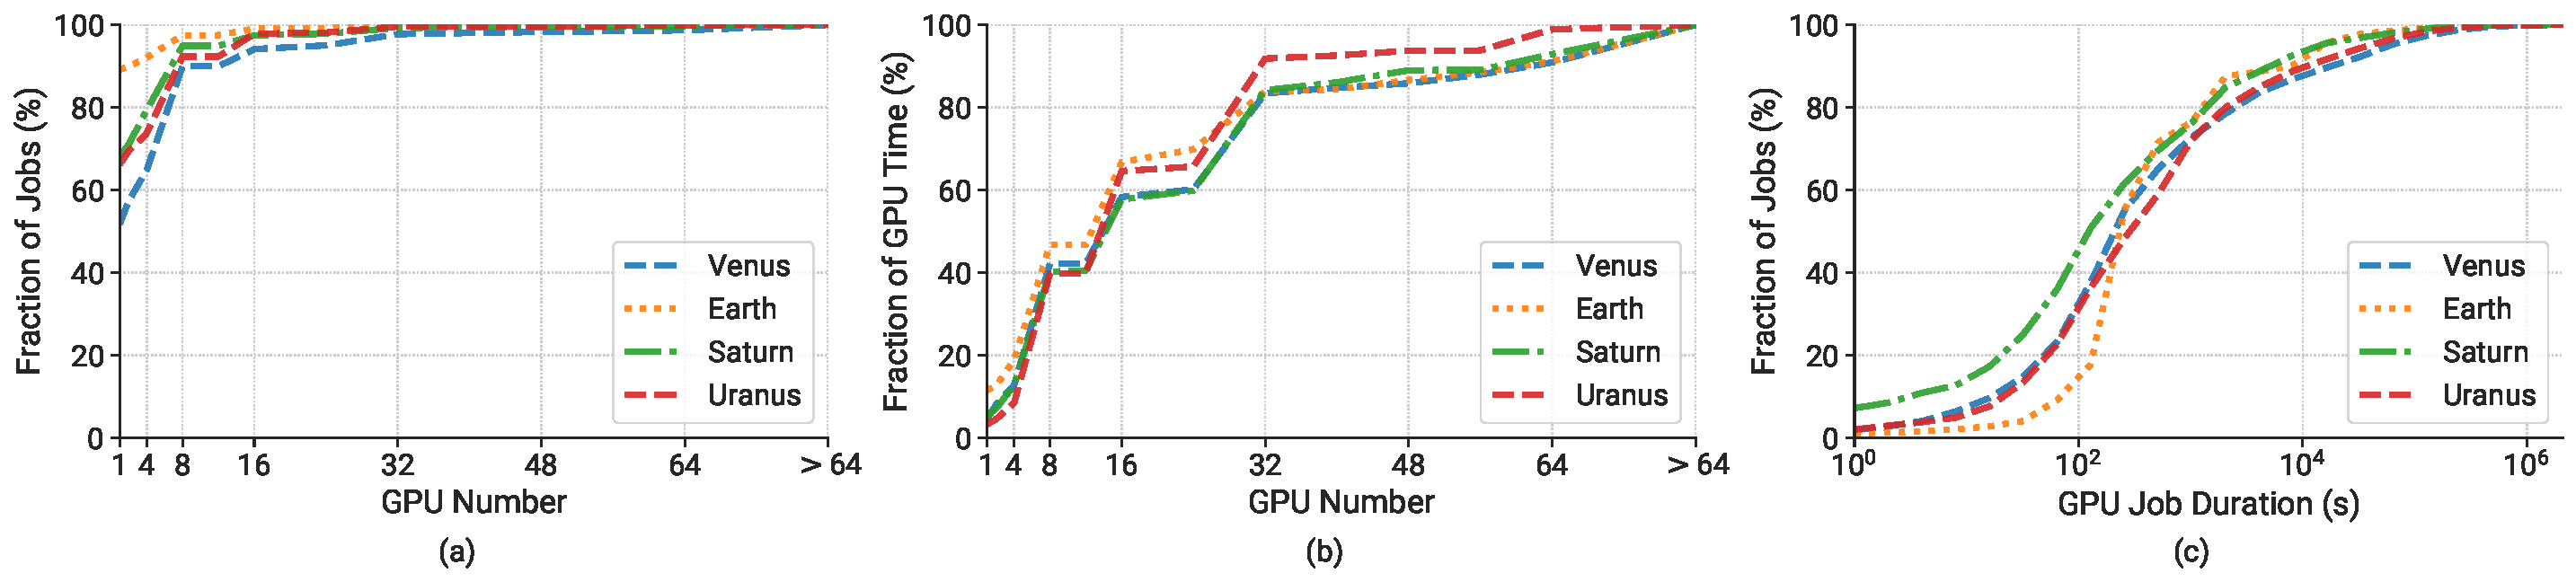
\includegraphics[width=\textwidth]{fig/dc_character}
    \vspace{-20pt}
    \caption{\textbf{Characterization of four clusters in SenseTime GPU datacenter Helios}. (a) CDF of job size with job distributions. (b) CDF of job size with GPU time distribution.  (c) CDF of job duration.}
    \vspace{-15pt}
    \label{figure_character}
\end{figure*}

\subsubsection{Challenges for Scheduling Training Jobs}
\label{subsec_challenge_training}
As discussed in Sec. \ref{sec:training-feature}, DL training workloads have some unique requirements compared to HPC or cloud jobs, which raises some challenges for scheduling them. We discuss these challenges with a workload trace analysis from four private clusters (\emph{Venus}, \emph{Earth}, \emph{Saturn} and \emph{Uranus}) in SenseTime GPU datacenter \texttt{Helios} \cite{Helios}. These clusters contain over 6000 GPUs and 1.5 million GPU jobs in total, spanning 6 months in 2020. 



\textbf{C1: Intensive resource consumption}. The adoption of distributed training aims to reduce the training time yet prompts users to overclaim GPU resources for their jobs.
Figures \ref{figure_character} (a) and (b) depict the distributions of requested GPUs pertaining to job and GPU resource occupation respectively. We observe that large-size jobs ($\leq$8 GPUs) account for 10\% of the entire trace, and they consume over half of computing resources. Such intensive resource requests can aggravate the job pending issue due to the shortage of GPU resources. If the scheduler prioritizes those large-scale jobs, the situation becomes worse as subsequent jobs have to compete for much less resources. Existing solutions often favor small jobs or treat large and small jobs equally. How to balance the trade-off between intensive and light-weight resource consumption remains a challenging problem.

\textbf{C2: Unbalanced runtime distribution}. Recent trace analysis works \cite{Philly, Helios, AliPAI, MLaaS} presented the long-tail runtime distribution of DL training workloads in production GPU datacenters. Figure \ref{figure_character} (c) compares the GPU job duration distribution of each cluster. We observe it is common that job runtime varies from seconds to weeks even months among different production-level GPU clusters. The majority of workloads only finish within a short period of time, while the minority part consume many orders magnitudes of GPU time. Prioritizing short jobs is an effective way to reduce average job completion time but incurs low GPU utilization. More research efforts should be devoted to balance between short jobs and time-consuming jobs.

\textbf{C3: Heterogeneous resource affinity}. The runtime speed of a DL training job is affected by a variety of hardware factors, among which GPU heterogeneity and network link heterogeneity are the most important ones. For the impact of GPUs, DL training can benefit from newer generations of GPUs. However, the marginal benefit brought by new GPU versions varies significantly (Figure \ref{figure_illustrate} (f)). Also, the speedup ratio is unpredictable, which complicates the heterogeneous GPU resource allocation. For the impact of network links, the recently released high-end GPU interconnect including NVlink and NVswitch can significantly reduce the communication overhead across GPUs in the same sever. Along with PCI Express, InfiniBand, Ethernet and QPI, distributed training has several alternatives for cross-GPU communications. As these links differ considerably in bandwidths, and different jobs have different data sizes for exchange, it is non-trivial to allocate these network resources to the jobs to maximize the benefits and minimize the bandwidth contention.


\textbf{C4: Preemption overhead}. DL frameworks usually provide functions to pause/resume the training jobs at any time for better fault-tolerance. The overhead of such processes primarily depends upon the job scale, which ranges from seconds to minutes. In this paper, the preemption overhead is considered as the addition of the costs of pausing and resuming the job. For time-consuming jobs, the preemption overhead is relatively small with the benefit of higher scheduling flexibility. But for short jobs, the preemption overhead is non-negligible, and frequent preemption will delay their progress. Designing an appropriate preemptive mechanism requires meticulous considerations of both short and time-consuming jobs as well as their preemption overheads.

\subsubsection{Challenges for Scheduling Inference Jobs.}
\label{sec_inference_challenge}The online execution fashion and high latency requirement of inference workloads also give the following challenges for designing a scheduler.


\textbf{C5: Low GPU utilization for each request.}
Compared to training jobs, the inference service mainly involves small convolutional operations (e.g., 1x1, 3x3), and consumes small amounts of GPU resources. Besides, the peak performance of new GPUs are increasing rapidly~\cite{IOS}. This often leads to low GPU utilization for inference workloads \cite{lemay2020Perseus,zhang2020mark}. A common practice to improve the GPU utilization is to batch multiple inference requests and execute them at the same time \cite{Daniel2017clipper}.



\textbf{C6: Latency-accuracy-cost tradeoff.}
The inference jobs are relatively malleable in terms of latency, accuracy and cost. To improve the resource utilization and cluster-wide job throughput, we can colocate multiple inference jobs or increase the batch size. However, this can increase the inference latency. To increase the accuracy, effective ways include model ensemble or augmentation evaluation, which can also incur latency delay \cite{Jashwant2021Cocktail}.
The adoption of high-class hardware resources can accelerate the inference execution, but charges more for online services. Different users or inference jobs may have different demands towards latency, accuracy and cost. The scheduler needs to figure out a sweet spot for each job over an assortment of algorithms and hardware units.



\textbf{C7: Bursty and fluctuating requests.}
As an online service, it is common for the inference application to receive bursty and fluctuating requests, which are unpredictable. This must be considered when determining the resources for the workload. How to guarantee the latency with the minimal operational cost even in extremely overloading scenarios raises a new challenge. In practice, resources are often over-provisioned for inference workloads to guarantee their latency during the rush hours. Then an efficient scheduler needs to consider how to exploit the unused resources of these workloads when there are less queries.












\subsection{Relevant Studies Not Included in This Survey}






This survey mainly focuses on the scheduling of DL training and inference workloads in GPU datacenters. Other relevant works beyond the scope of this paper will not be summarized in the following sections. Here we briefly discuss these directions. Readers who are interested in these works can refer to relevant surveys \cite{SurveyDistDL, SurveyDML,SurveyPruneQuant, SurveyInfer21,SurveyCloudSched, SurveyCloudSched17,SurvHPC, SurveyHPCBigData}.







First, we do not consider the \textit{optimization solutions} for \textit{individual} training or inference jobs. Training job optimization mainly contains distributed training acceleration \cite{BytePS, Poseidon, LB-BSP} and job placement optimization \cite{HeteroG, Pack, OJPP}. Inference job optimization techniques include workload characterization~\cite{chahal2021performance}, pipeline execution~\cite{kang2020jointly}, etc. Their objectives are to achieve high performance for a single job instead of an entire datacenter.  It is worth noting that scheduling hyperparameter optimization jobs will not be considered as single job optimization, because it involves a collection of training tasks (e.g., RubberBand \cite{RubberBand}, HyperSched \cite{HyperSched}). They will be summarized in Sec. \ref{sec_other_workload}.

Second, we consider the scheduling at the job level, and do not cover the scheduling approaches at the hardware resource level (e.g., network I/O, power). For instance, HIRE \cite{HIRE} proposed a novel in-network computing scheduling algorithm for datacenter switches. A number of works \cite{DVFS-AWARE, mei2021energy, DVFS2020} utilized the DVFS mechanism on CPU and GPU chips to achieve cluster energy conservation. These works are not included in this survey.

Third, we focus on the GPU datacenters where GPUs are the primary resources for the DL workloads. Those datacenters can also exploit other resources (e.g., CPU, FPGA, ASIC) as subsidiary. This can reflect the current status of mainstream DL infrastructures. Some scheduling systems mainly utilize the CPU~\cite{yan2016SERF,Ishakian2018Serving,Bhattacharjee2019BARISTA,Gunasekaran2020Fifer}, FPGA~\cite{jiang2021MicroRec,hwang2020Centaur}, or hybrid resources~\cite{jiang2021FleetRec} where GPUs are not dominant. Some papers consider the DL services on mobile devices~\cite{Ogden2021PieSlicer} or edge computing~\cite{seo2021SLO_Aware,zhang2020QoS} other than datacenters. Those works are also out of the scope of this survey.



Fourth, we target the scheduling of general DL training and inference workloads. Some works studied other types of DL jobs, e.g., data processing, model re-training, model validation. Some papers considered the optimization of specific DL applications based on their unique behaviors, including RNN-based service~\cite{gao2018low,holmes2019grnn}, recommendation systems~\cite{gupta2020deeprecsys, liu2021jizhi,jiang2021MicroRec,jiang2021FleetRec} and video analytics~\cite{shen2019nexus,zhang2020hysia}. These works are not summarized in this paper. Besides, our aim is to enhance the system and workloads in terms of performance, efficiency and user experience. Other objectives like privacy protection~\cite{DPF,Sage} is not considered either.




























